\part{Des sources utiles}

\chapter{Blogs de français à l'étranger}

\section{Le blog d'un voyageur}

\paragraph{} ``Le blog de Didier // Voyageur dans l'âme'' \\
Ce blog retrace les voyages de Didier, un français qui aime beaucoup voyager.
Il y raconte ce qu'il a vu, ses impressions ainsi que de bonnes adresses. On
peut aussi y trouver des conseils concernant l'organisation du voyage tel que
la liste des préparations indispensables avant de partir, des idées d'activité
ou encore comment choisir son appareil photo.

\begin{center}
	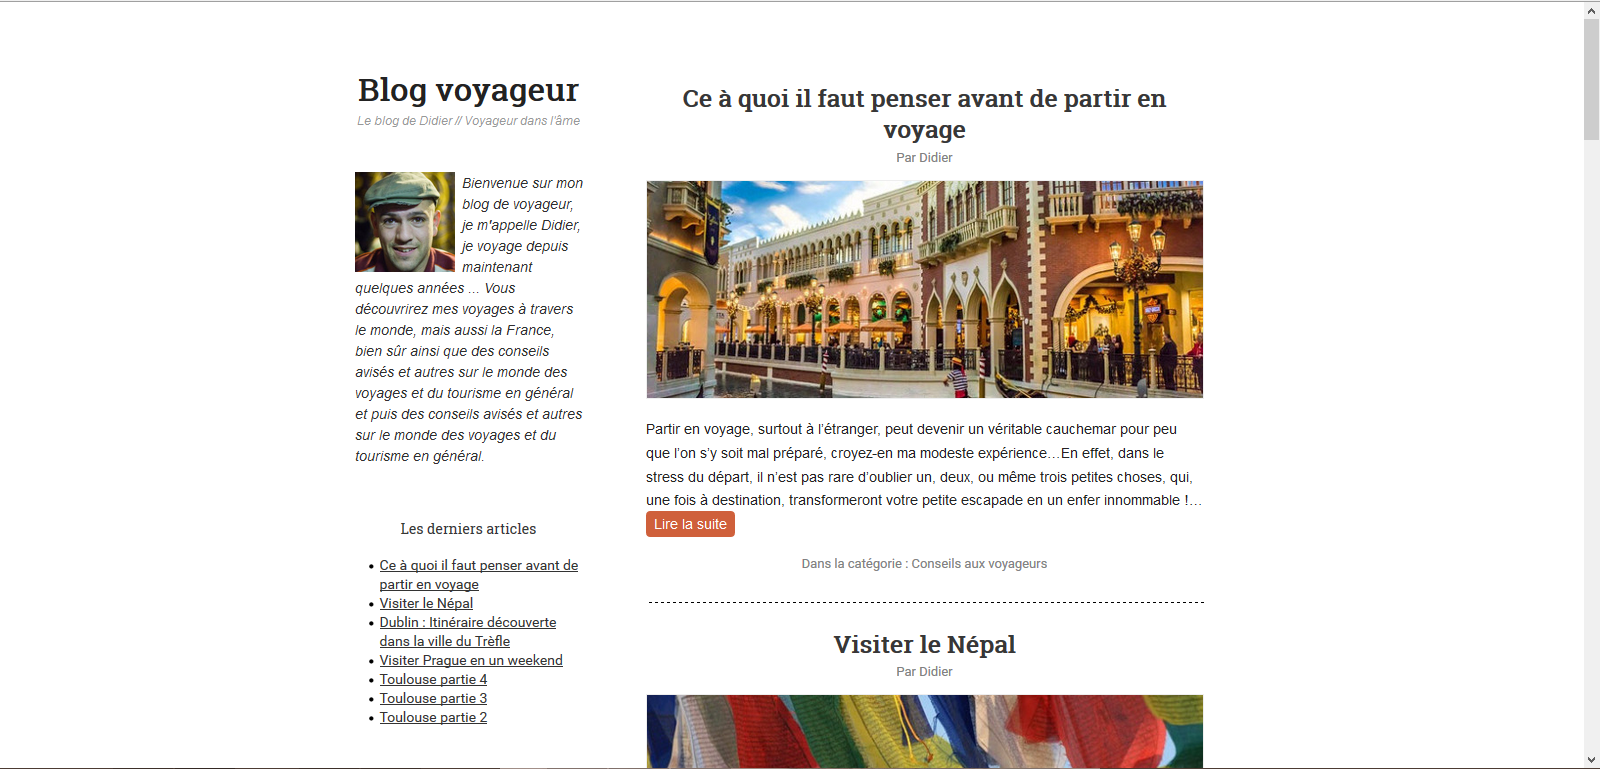
\includegraphics[scale=0.25]{voyageur.png}
\end{center}
\url{http://www.blogvoyageur.fr/}

\section{Le comptoir de Toamasina}

\paragraph{} Jeune Français de 26 ans, qui vit entre la France et le Brésil
depuis 2 ans. Après 3ans dans l'importation de vanille et la découverte de la
grande île, le voici dans ce nouveau continent où il posera ses valises
définitivement il y a 12 mois.

\begin{center}
	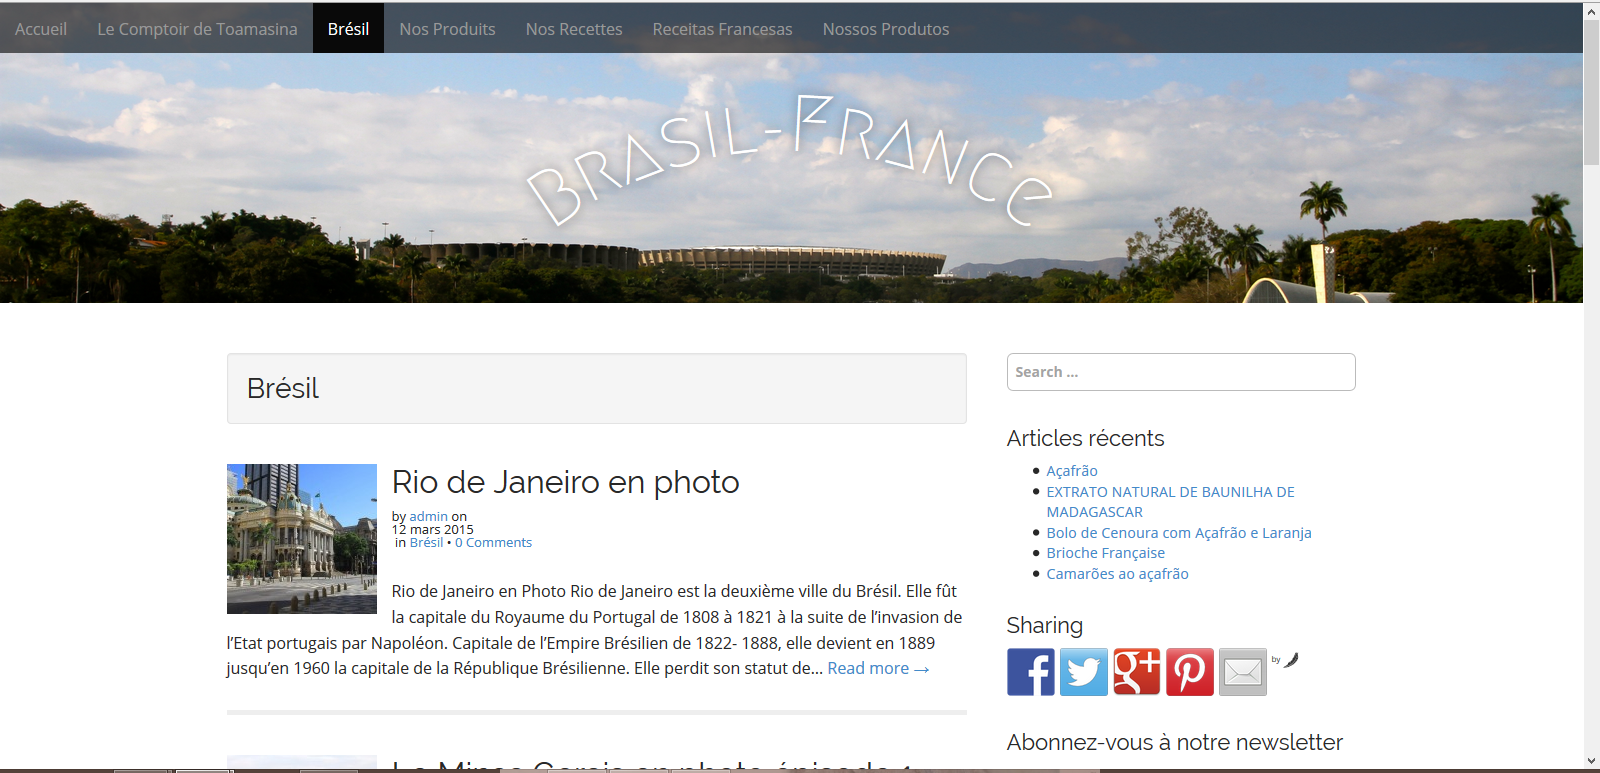
\includegraphics[scale=0.25]{Toamasina.png}
\end{center}
\url{http://lecomptoirdetoamasina.fr/brasil-france/category/bresil/}

\section{Expérience nippone}

\paragraph{} Il s'agit du blog de Svetlana Zehnder, une jeune femme française
de 25 ans qui réside au Japon à Osaka depuis 2014. Elle y raconte ses
expériences, ce qui l'étonne dans cette culture et des nouvelles du Japons.

\begin{center}
	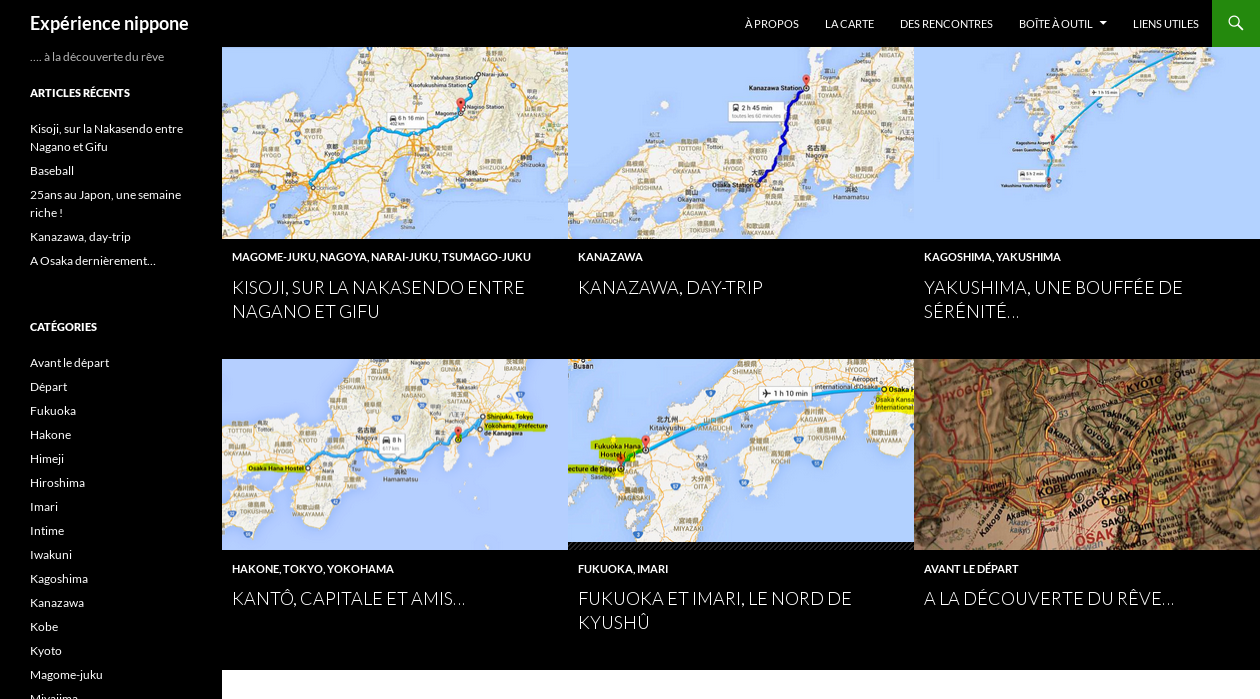
\includegraphics[scale=0.25]{Svetlana.png}
\end{center}
\url{https://svetlanainjapan2014.wordpress.com/}

\chapter{Blogs d'étranger en France}

\section{Un américain en France}

\paragraph{} Ce blog est tenu par Jim, un américain originaire d'Atlanta vivant
en France. Il y poste des articles et des vidéos comparant la culture française
et la culture américaine. Il répond aux questions souvent posées par les
français notamment celles postées sur son blog.

\begin{center}
	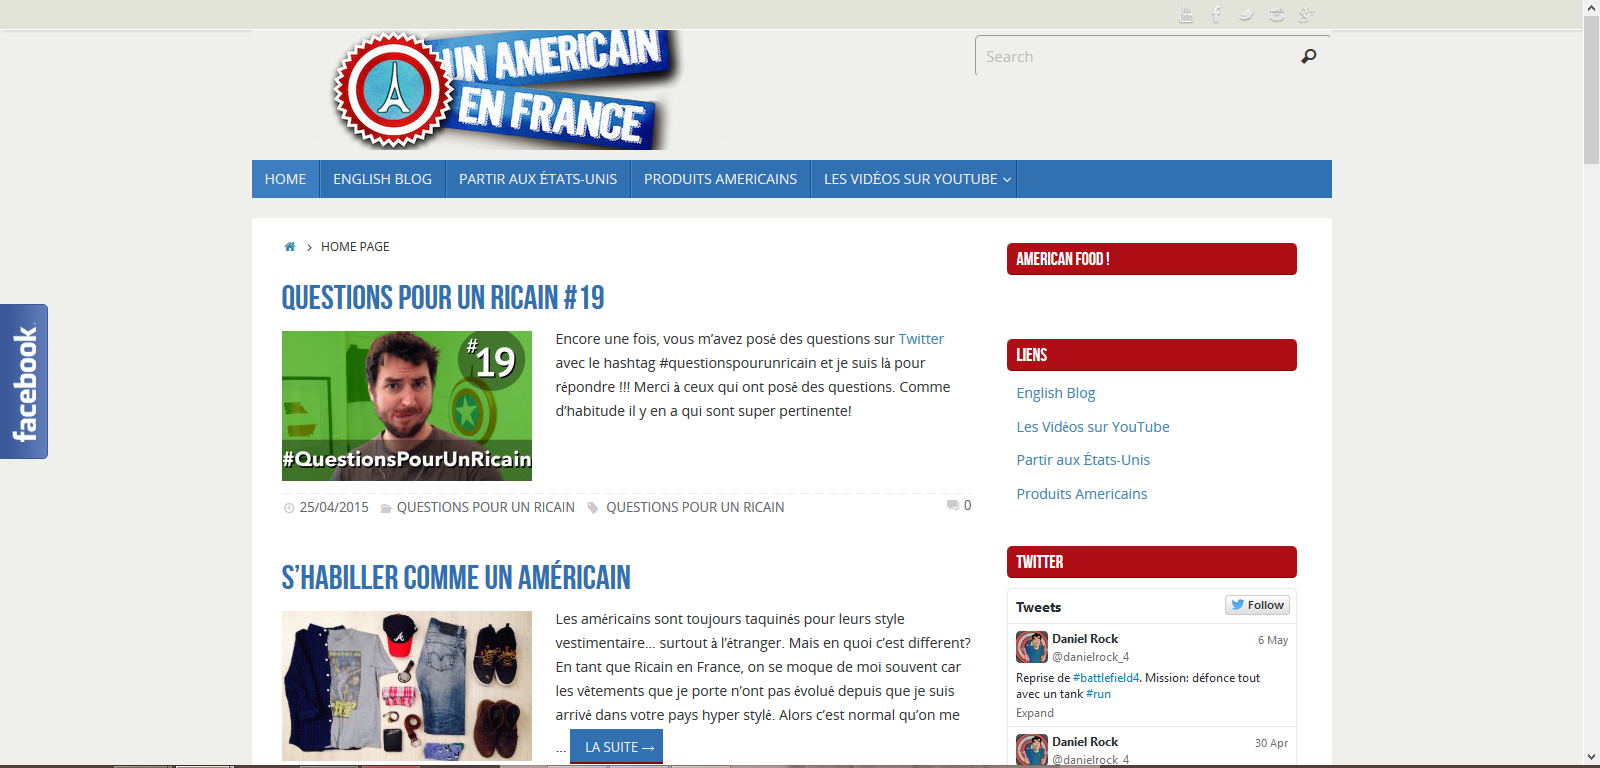
\includegraphics[scale=0.25]{Americain.png}
\end{center}
\url{http://unamericainenfrance.com/}

\section{À fond de France}

\paragraph{} Venus d’Algérie, du Burkina-Faso, de Côte d’Ivoire, de Chine, de
Colombie, du Japon, de la République Démocratique du Congo et de Russie, ils
s’apprêtent à asser trois ans en France pour y étudier le journalisme. À
Fond-de-France, dans la vallée du Haut-Bréda, ils vont découvrir un petit bout
de leur pays d’accueil.

\begin{center}
	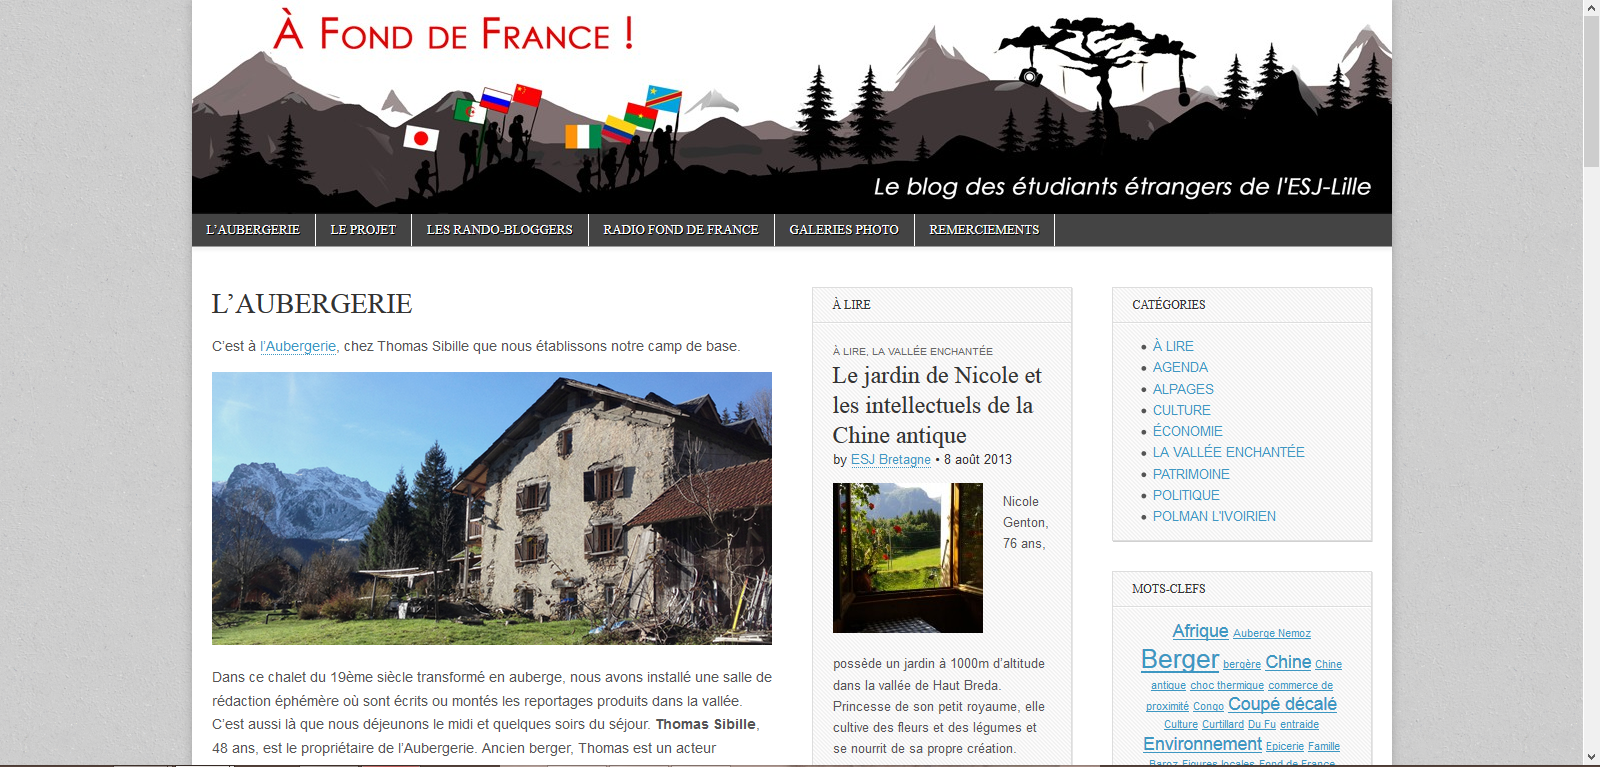
\includegraphics[scale=0.25]{AFondDeFrance.png}
\end{center}
\url{http://fonddefrance.esj-lille.net/laubergerie/}

\section{Rejected in Paris}

\paragraph{} Ce blog raconte les expériences d'un écrivain américain renommé,
écrivant un roman à succès, qui se trouve exclu à Paris de différente manière.
Il y décris sa vie, ses exclusions et leurs raisons.

\begin{center}
	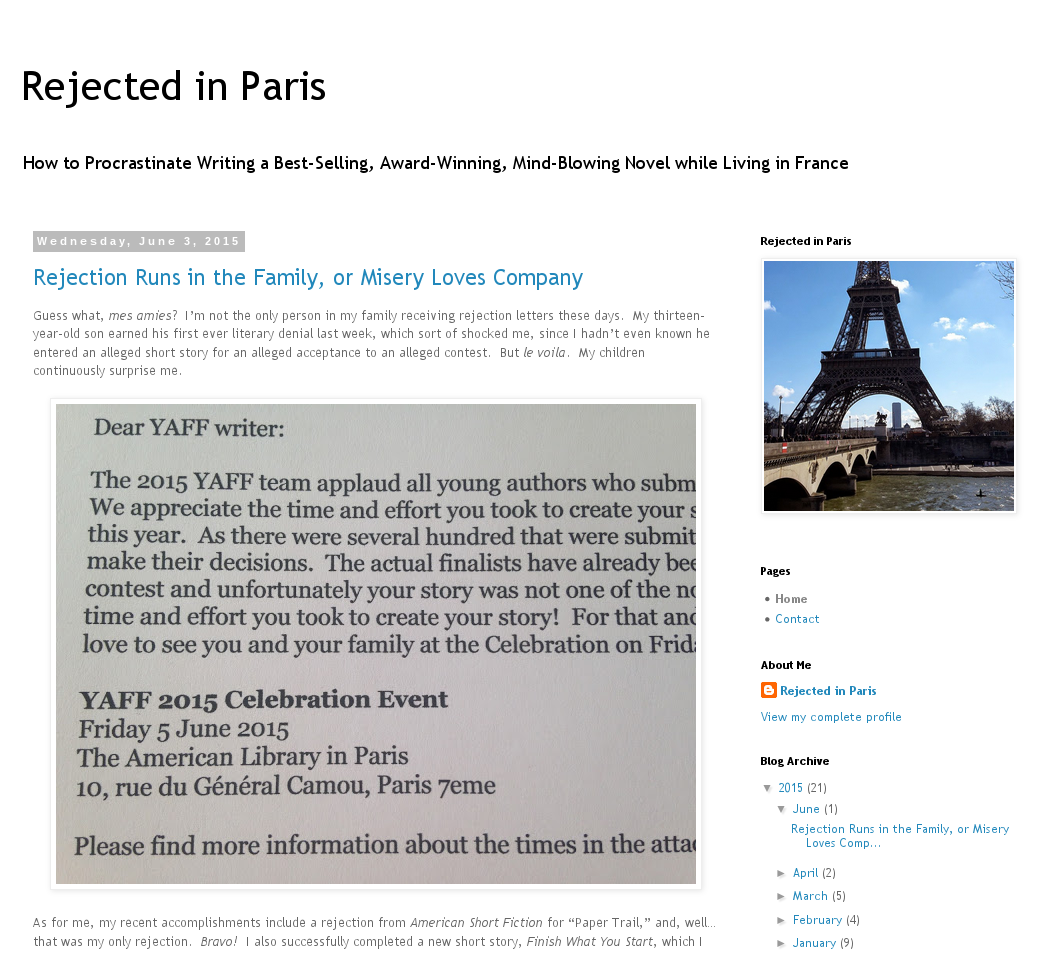
\includegraphics[scale=0.25]{Rejected.png}
\end{center}
\url{http://www.rejectedinparis.com/}

\chapter{Sites sur l'interculturalité}

\section{About interculturalisme}

\paragraph{} Ce site a été créé par Ted Cantle. C'est un écrivain ayant écrit
deux livres sur l'interculturalité. Ce site comporte des informations sur
l'interculturalité  qui constitue une partie des recherche de cet écrivain.

\begin{center}
	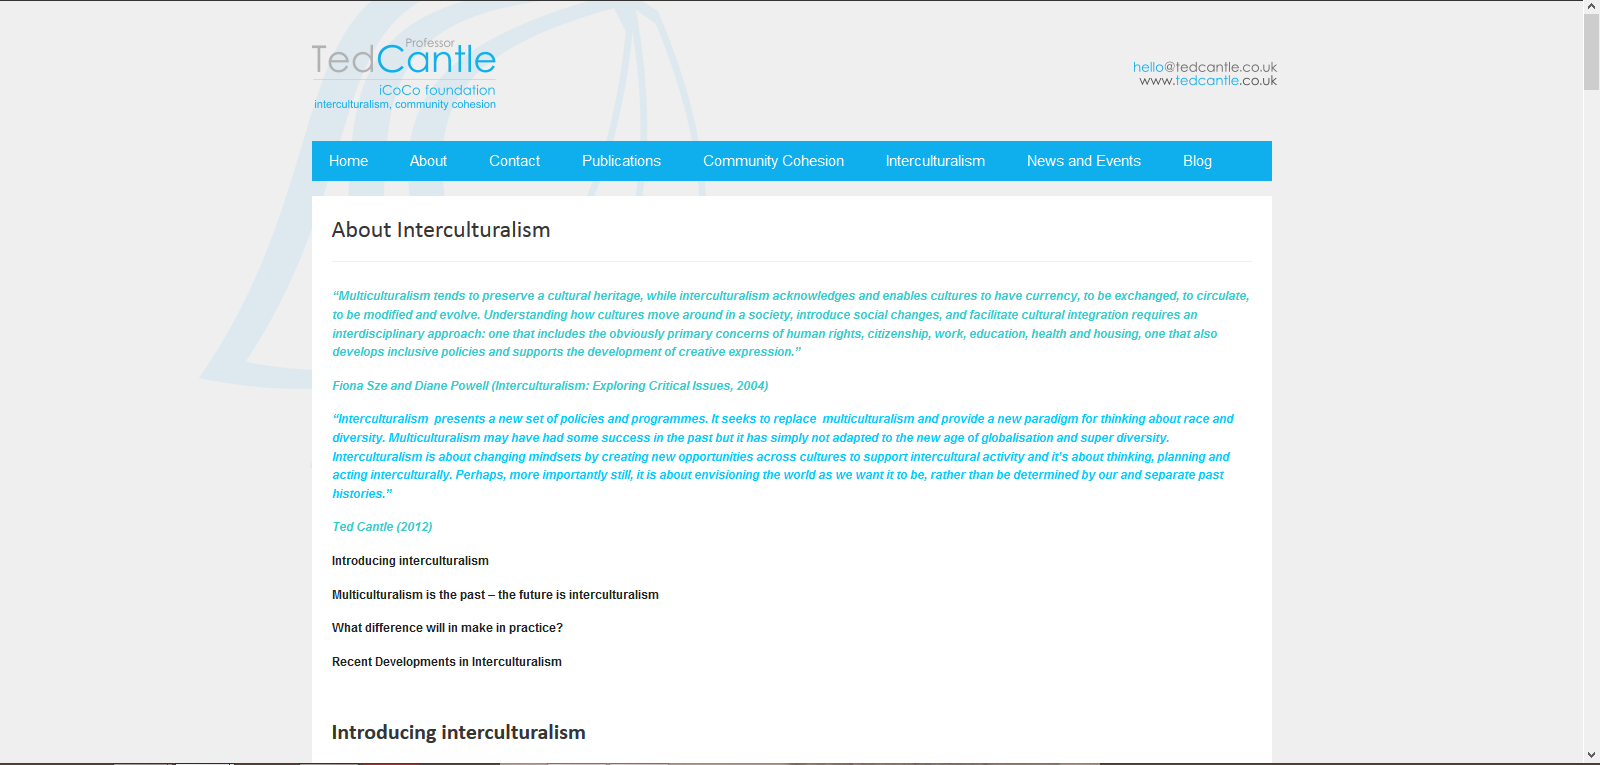
\includegraphics[scale=0.25]{interculturality.png}
\end{center}
\url{http://tedcantle.co.uk/publications/about-interculturalism/}

\section{La communication interculturelle}

\paragraph{} Blog d’une étudiante faisant des recherches et analyses sur
l’interculturalité. De nombreux sujets y sont abordés et il y a beaucoup de
chose à apprendre. Très théorique, ce blog se veut éducatif et espère que
chaque lecteur se fera un plaisir d’y faire un tour.

\begin{center}
	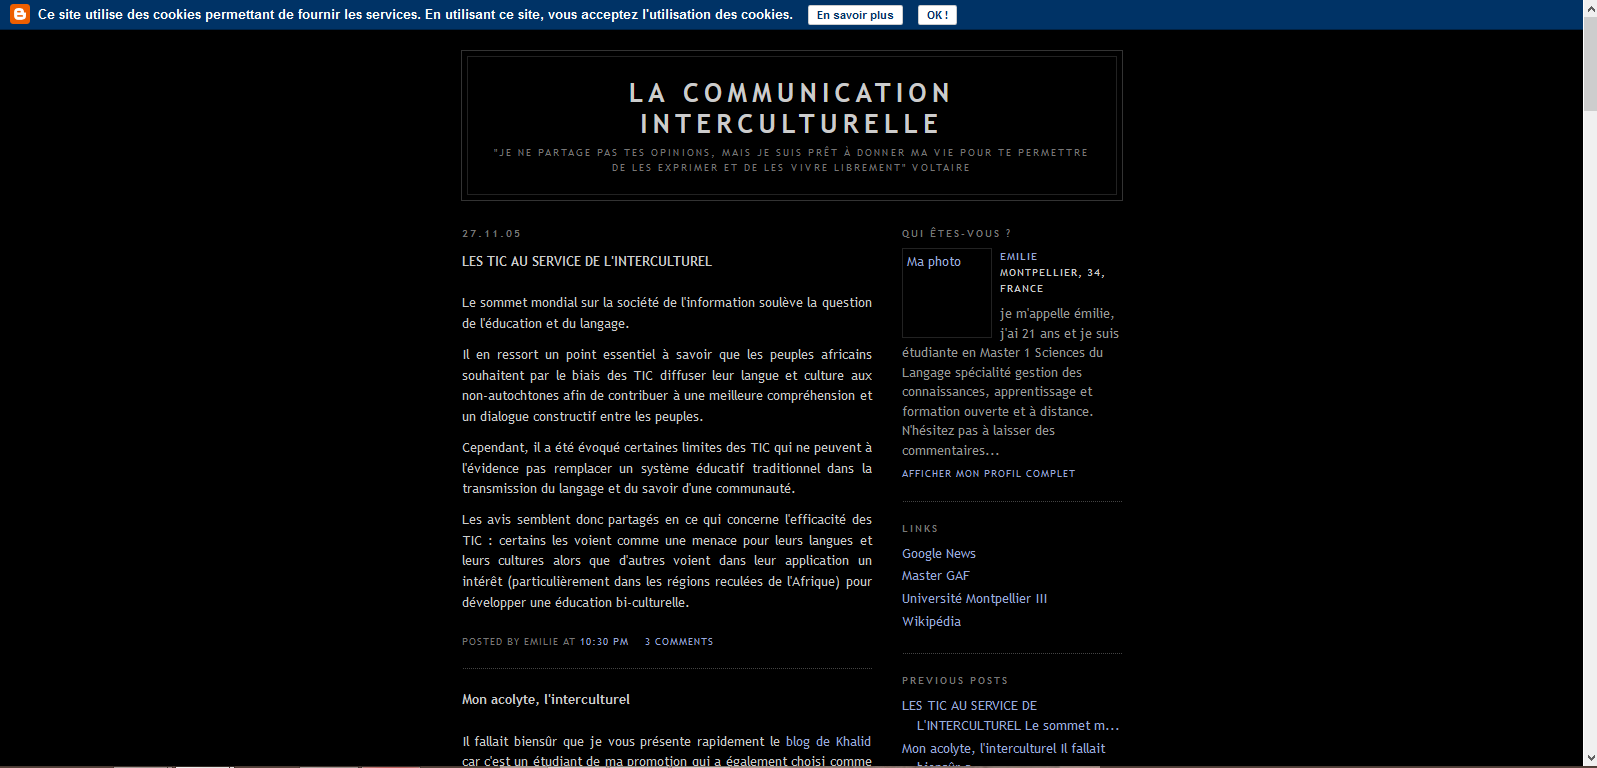
\includegraphics[scale=0.25]{ComInter.png}
\end{center}
\url{http://robertemilie3034.blogspot.fr/}

\section{ICI}

\paragraph{} Il s'agit du site de l'Institut de Communication Interculturelle.
On y trouve des informations sur comment communiquer lors de situations
pouvant engendrer des différences culturelles et des livres contenant d'autres
informations concernant l'interculturalité en général.

\begin{center}
	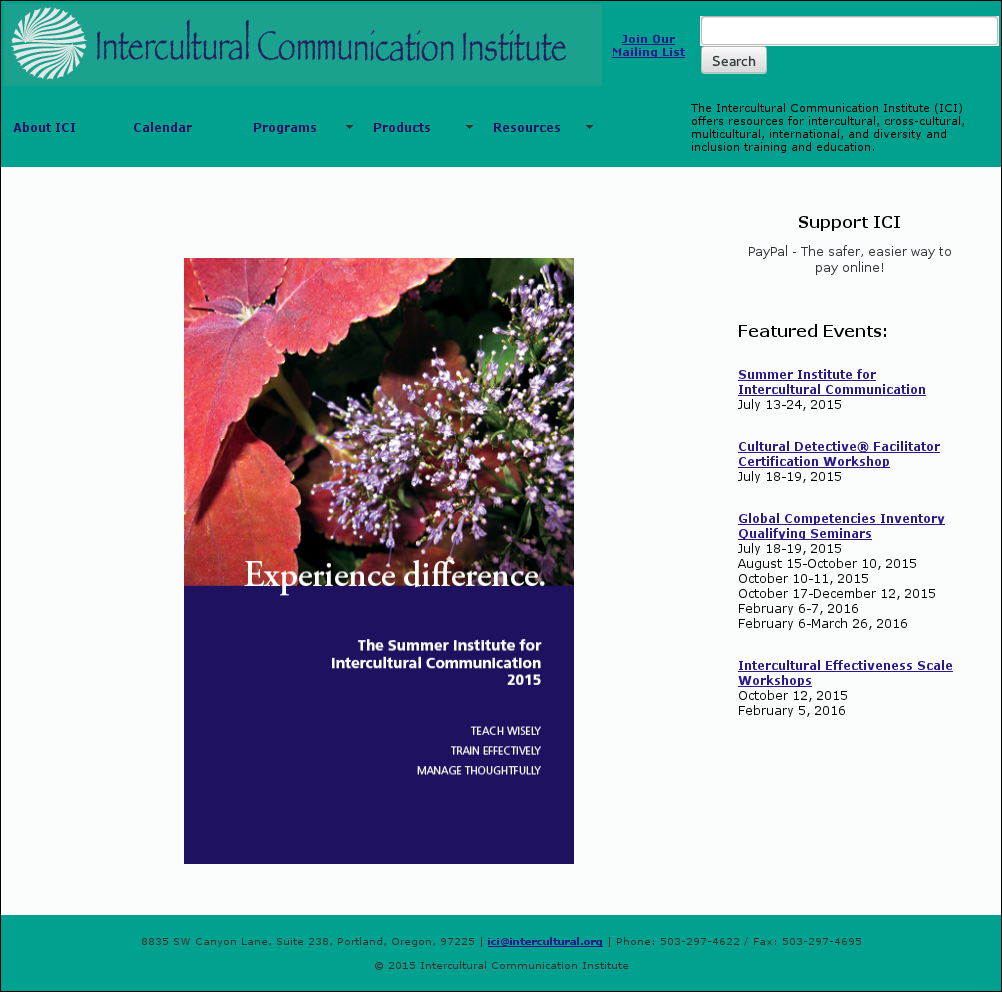
\includegraphics[scale=0.25]{Intercultural.png}
\end{center}
\url{http://www.intercultural.org/}

\chapter{Nos sources pour ce dossier}

\section{A chacun sa culture qui fait rêver}

\subsection{Le Brésil}
\noindent
\url{http://www.brasilpassion.com/culture-bresilienne.html}

\subsection{Le Japon: Matsuris et Croyances}
\noindent
\url{http://www.japan-guide.com/e/e2063.html}\\
\url{http://fr.wikipedia.org/wiki/Matsuri}\\
\underline{Le Japon des Japonais} par Philippe \textsc{pons} et Pierre-François \textsc{souyri}, édition L'autre guide

\section{Les Otakus ou les passionnés de mangas}

\subsection{Histoire du manga}
\noindent
\url{http://www.france-jeunes.net/lire-le-manga-et-la-france-analyse-d-un-succes-25649.htm}\\
\url{http://hitek.fr/actualite/dossier-manga-naissance-arrivee-france_1924}

\subsection{Vocabulaire}
\noindent
\url{https://en.wikipedia.org/wiki/Glossary_of_anime_and_manga}\\
\url{https://www.asianfanfics.com/blog/view/411262/url}

\subsection{Les produits dérivés}
\noindent
\url{http://www.lapinourose.com/}\\
\url{http://www.countrynavigator.com/ecr/ecr_japan_report_french.pdf}\\
\url{http://www.20minutes.fr/economie/1243001-20131029-20131029-animation-japonaise-exporte-bien-produits-derives}

\section{Concepts théoriques}

\subsection{Monochronique et Polychronique}
\noindent
\url{http://www.managementinterculturel.com/outils/rapport-temps.html}\\

\subsection{Communication haut contexte et bas contexte}
\noindent
\url{Wikipédia (en) - High- and low-context cultures}\\

\subsection{4 Dimensions culturelles}
\noindent
\url{http://geerthofstede.nl/dimensions-of-national-cultures}\\
\url{http://news.telelangue.com/en/2011/09/cultural-theory}
